\documentclass[a4paper,12pt]{article}
\usepackage[a4paper,margin=1in,footskip=0.25in]{geometry}
\usepackage[utf8]{inputenc}

% science
\usepackage{amsmath}
\usepackage{array}
\usepackage{siunitx}

% layout
\usepackage{float}
\usepackage{parskip}
\usepackage{graphicx}
\usepackage{circuitikz}
\usepackage{longtable}
\usepackage{hyperref}

% referencing
\usepackage[style=apa]{biblatex}
\addbibresource{light.bib}
\usepackage{hyperref}

% table centering
\renewcommand{\arraystretch}{1.3}
\newcolumntype{P}[1]{>{\raggedright\arraybackslash}p{#1}}
\newcommand{\tptt}{$\times\,$}

% figures labelings
\usepackage{chngcntr}
\counterwithin{figure}{section}

% uncertainty
\newcommand{\absun}{\Delta \text{un}\,}
\newcommand{\relun}{\% \text{un}\,}

\title{Empirically finding the typical luminous efficiency of a light bulb through the inverse square law}
\author{Terry Qi}

\begin{document}

\maketitle

\section{Design}

\subsection{Introduction}
% personal
During the examination of a potential IA idea on the intensity of a refracted light-beam, I struggled with the implementation of a realistic light due to a lack of understanding and care towards the drop of intensity of light with respect to the distance. Because the glass cube I was working with had significant length, the decrease in intensity of the light-beam within the glass damaged my data and exponentially increased the difficulty in linearization. Therefore, I wanted to empirically see how the difference in distances will affect the measurement of light intensity. Additionally, I found the labs bulbs are prone to extreme heat even with little power and duration. Thus, I thought to use this experiment to find the luminous efficiency of the typical light-bulbs to confirm my suspicion.

\subsection{Research Question}
\begin{quote}
 What is the relationship between the distance to the light source in respect to the perceived illuminance?
\end{quote}

\subsection{Background}

For a light-bulb to produce light, an electrical current in the form of moving electrical charges must be presented and pass through a light emitting electrical resistor. While there exists difference in the efficiency of such resistors --- modern light emitting diodes (LED) are much more energetically efficient comparing to an incandescent light-bulb, the physical result needed to illuminate a room through the emission of light waves in the visible spectrum, does not differ. Therefore, the theoretical definition of the rate of work, $P$, is only depended upon the level of electrical current (the flow rate of charges), and voltage (the work potential of charges), shown in figure \ref{eq:work}.

\begin{figure}[h!]
    \[
    P = IV
    \]
    \caption{The electrical definition of work}
    \label{eq:work}
\end{figure}

For it is the emission of light waves/photons that we call ``light'', the density of these photons in an area naturally defines the intensity of light (of units $\si{W\per m^2}$). This relationship is a part of the IB curriculum at topic 4.3, Waves Characteristics, where it states a fundamental property of light intensity --- that the intensity of light is proportional to the inverse distance squared (figure \ref{eq:prop}).

\begin{figure}[h!]
    \[
    I \propto \frac{1}{s^2}
    \]
    \caption{The inverse square relation}
    \label{eq:prop}
\end{figure}

Furthermore, if we consider the emission of these photons to be a perfect sphere around the light source, the density of photons at a given distance is simply represented via the surface area of the sphere with a radius of the distance.
%images
Using the unit definition of intensity, we can derive using the equation of the surface area of a sphere, the full intensity equation in figure \ref{eq:isl}:

\begin{figure}[h!]
    \[
    I = \frac{P}{\text{Area}} = \frac{P}{4\pi s^2}
    \]
    \caption{The inverse square law}
    \label{eq:isl}
\end{figure}

However, the human eyes does not perceive the intensity of light uniformly through the wavelengths (citation). Under conditions for photopic vision --- the vision of the eye in a well lit area, we perceive light in the green wavelength (555 $\si{nm}$) the most intensely. Therefore there is a need for a unit that displays the normalized intensity of different wavelengths of light --- the unit Candela and the photopic luminosity function.

% talk about the relationship between
The intensity derived from the inverse square law (figure \ref{eq:isl}) is more formally known as the \textit{radiant intensity} (citation), represented as a function of wavelength: $I_v(\lambda)$. By taking the incomplete integral on the weighted radiant intensity split into frequencies for all frequencies, we come to the definition of the \textit{luminous intensity} $I_v$, shown in figure \ref{eq:li}.

\begin{figure}[h!]
    \[
     I_v = K_{cd} \int_{0}^{\infty} V(\lambda) I_e(\lambda) \, d\lambda
    \]
    \caption{The definition of Luminous Intensity}
    \label{eq:li}
\end{figure}

Combining the notion of luminous intensity with the 3D generalized angle quantity, steradian ($\si{\ohm}$), we can derive the total luminous power ($\Phi_v$) created by the source, measured in unit lumen ($\si{lm}$),

\[
    \Phi_v = \si{\ohm} I_v,
\]

of which we can use to define the amount of luminous power incident on a surface through the quantity of illuminance, measured in units lux ($\si{lm\per m^2}$). The finalized relation is summarized in figure \ref{eq:dti}:

\begin{figure}[h!]
 \centering
 \begin{align*}
 I_e(\lambda) &= c(\lambda) \frac{P}{4\pi s^2}\\
  E_v &= \frac{1}{4\pi s^2 A} \si{\ohm} P K_{cd} \int_{0}^{\infty} V(\lambda) c(\lambda) \, d\lambda\\
  E_v & \propto \frac{1}{s^2}
 \end{align*}
 \caption{The complete distance to illuminance relationship}
 \label{eq:dti}
\end{figure}


For the light sensor used in the experiment measures intensity in lux, the above dive into luminosity serves as a justification for why I think the inverse square root applies to not just radiant intensity, but also to luminous intensity. Because the process of conversion is linear, it seems reasonable to hypothesise that illuminance is proportional to the distance squared.


\subsection{Variables}
\paragraph{Independent Variable}
The distance the light sensor is to the light source measured in centimeters.

\paragraph{Dependent Variable}
The illuminance of the area measured by the light sensor at the distance in unit lux.

\subsection{Control Variables}

\begin{longtable}{P{0.2\textwidth}|P{0.35\textwidth}|P{0.35\textwidth}}
Controls & Reason & How\\\hline
Environmental room intensity & Systematically increase the the measured illuminance of the light-ray from the light-box & Conduct the experiment in a dark room, and record the ambient illuminance of the room \\
The sensitivity of the light sensor & Light sensors are sensitive to angular tilts, and a disturbed sensor due to shaky hands most likely will produce random errors throughout the experiment & Use strong tape to clamp down the light sensor at the given distance\\
Fluctuation of the outside light level & Environment lighting will leak through the lab windows, and have the ability to systematically change the measurements for a small time period & Conduct the experiment early in the morning or late at night, as to minimize the impacts from the sun\\
The power supplied to the light-bulb & Higher power will increase intensity at all distances, as shown in figure \ref{eq:isl}, causing systematic errors & Assert the connected ammeter and voltmeter readings are unchanged after changing the independent variable, the distance\\
The temperature of the bulb filament & For the resistance of a resistor tend to increase as it is heated, electrical current may fall in value, decreasing the power supplied, creating systematic errors & It is discouraged to directly touch the light-bulbs. Thus it is best to conduct the experiment quickly in time, as to minimize the possible heating up of the light-bulb.

\end{longtable}


\subsection{Materials}
\begin{itemize}
 \item Vernier light sensor \& connection hub
 \item laptop with Vernier Data Logger software
 \item 5W light-bulb
 \item 5 wires
 \item 12V power supply
 \item digital ammeter and voltmeter
 \item reasonable supply of duct tape
 \end{itemize}

\subsection{Method}

\begin{enumerate}
 \item Dim the room lights and choose a location with the least amount of ambient light to do the experiment. Ideally the test should be done early in the morning or at night.

 \item Connect the Vernier light sensor ($\pm$ 1 \si{lux}) to the connection hub, then to the laptop. Change the light sensor's range to (0–6000 \si{lux}) by flipping the side switch to the up position, and verify a reading within the software on the laptop. Enable ``Statistics'' in the software by clicking the button named ``Stats''.

 \item Set up the electrical circuit as shown in diagram \ref{fig:cd}, using a 5W light-bulb, 5 insulated wires, an 12V power supply dialled down to 8V, and a digital ammeter ($\pm 0.1 \si{A}$) and voltmeter ($\pm 0.1 \si{V}$). Note that the light-stand may need to be tilted so the light-bulb is in contract with the ground.

 \item Align the meter wooden ruler perpendicularly to the light-bulb, position the Vernier sensor unit along the long edge of the ruler at a distance of 3cm to the light-bulb. The final layout should be similar to figure \ref{fig:layout}.

 \item Secure down the light sensor using tape at distances of 3cm to 10cm, step 1cm, of a total of 8 distances.

 \item For each distance, first record the readings on the ammeter and voltmeter. If the readings fail to match that of the previous IV, retry the previous test. Wait for the illuminance value to stop fluctuating at a great scale, then press the ``record'' button in the Vernier logger software. Note down the mean illuminance value shown in a textbox from the recording in a spreadsheet. Repeat this recording of illuminance 5 times at the same distance while noting down their respective values.
\end{enumerate}

\subsection{Diagrams}

% circuit
\begin{figure}[h!]
\centering
\begin{circuitikz} \draw
    (0,3) to[battery,a=8V] (5,3) -- (5,0)
    to[lamp,a=5W] (0,0)
    to[ammeter] (0,3)
    (1,0) -- (1,-1.5)
    to[voltmeter] (4,-1.5) -- (4,0)
    ;
\end{circuitikz}
\caption{The circuit diagram of the setup}
\label{fig:cd}
\end{figure}

% diagram
% annotated picture, & a software screen
\begin{figure}[h!]
 \centering
 \caption{The experiment layout}
 \label{fig:layout}
\end{figure}


\subsection{Safety}
Avoid direct contact with exposed parts of the wires, additionally ensure a dry hand during the experiment. This will reduce the chance of an electrical accident.

Avoid touching the light-bulb throughout the experiment. The light-bulb got super hot during my experiment and direct skin contract may incur burns.

\section{Data}
\subsection{Raw data}
\begin{figure}[h!]
    \centering
    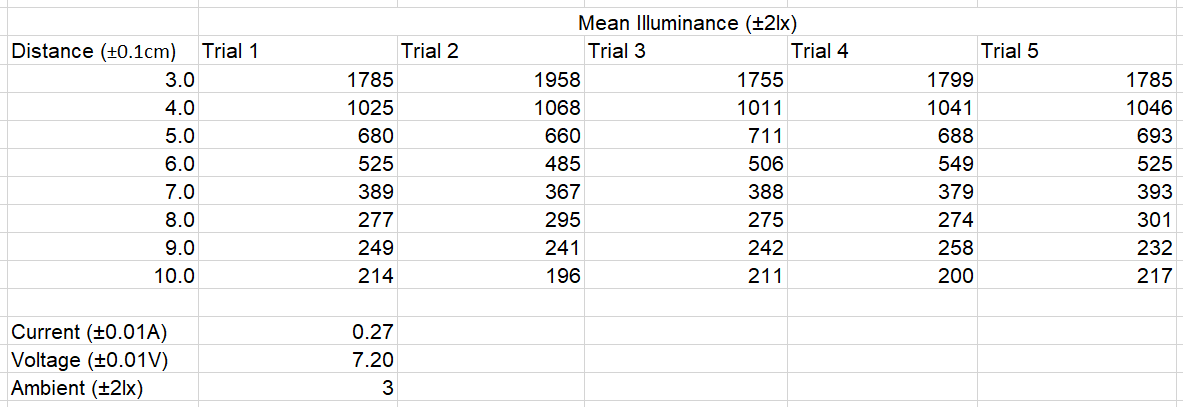
\includegraphics[width=\textwidth]{assets/rawdata.png}
    \caption{Unprocessed experimental data}
\end{figure}

\subsection{Processing}
\paragraph{Notation}

Uncertainty: un \quad Absolute uncertainty: $\Delta$un \quad Relative uncertainty: \%un


\subsubsection*{Processing Power}
Power is defined in figure \ref{eq:work}:
\begin{align*}
\text{Power} &= \text{Current} \times \text{Voltage}\\
        &= 0.27\si{A} \times 7.20\si{V} \approx 1.94 \si{W}
\end{align*}

\textit{Uncertainty}: \%un W = \%un A + \%un V
\begin{align*}
    \relun A &= \frac{0.01}{0.27},\quad \relun V = \frac{0.01}{7.20}\\
    \relun W &\approx 0.038,\quad \absun W \approx 0.07W
\end{align*}


\subsubsection*{Processing Illuminance}
Subtract the each illuminance values by the ambient illuminance value (figure \ref{fig:corrected}).

\textit{Uncertainty}: $\absun$Corrected = $\absun$Measured + $\absun$Ambient
\begin{align*}
     \absun \text{Corrected} = 0.2 + 0.2 = 0.4\si{lx}
\end{align*}

\begin{figure}[h!]
    \centering
    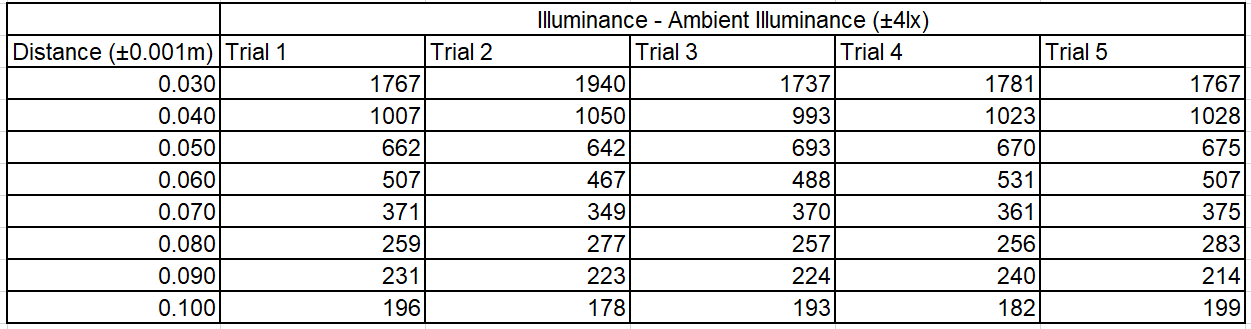
\includegraphics[scale=0.5]{assets/correcteddata.png}
    \caption{Corrected illuminance values}
    \label{fig:corrected}
\end{figure}

Average the measured illuminance. Additionally, the distances are converted into standard SI units in meters (figure \ref{fig:average}, graph \ref{gph:average}).

\begin{figure}
    \centering
    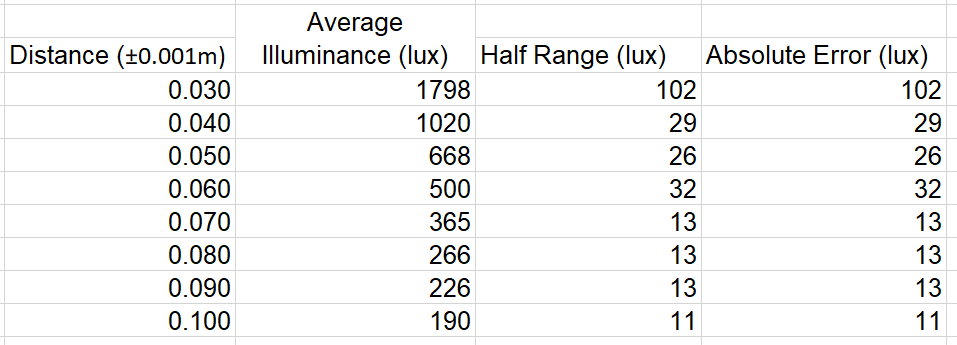
\includegraphics[scale=0.6]{assets/averagedata.png}
    \caption{Averaged illuminance values}
    \label{fig:average}
\end{figure}

\begin{figure}
    \centering
    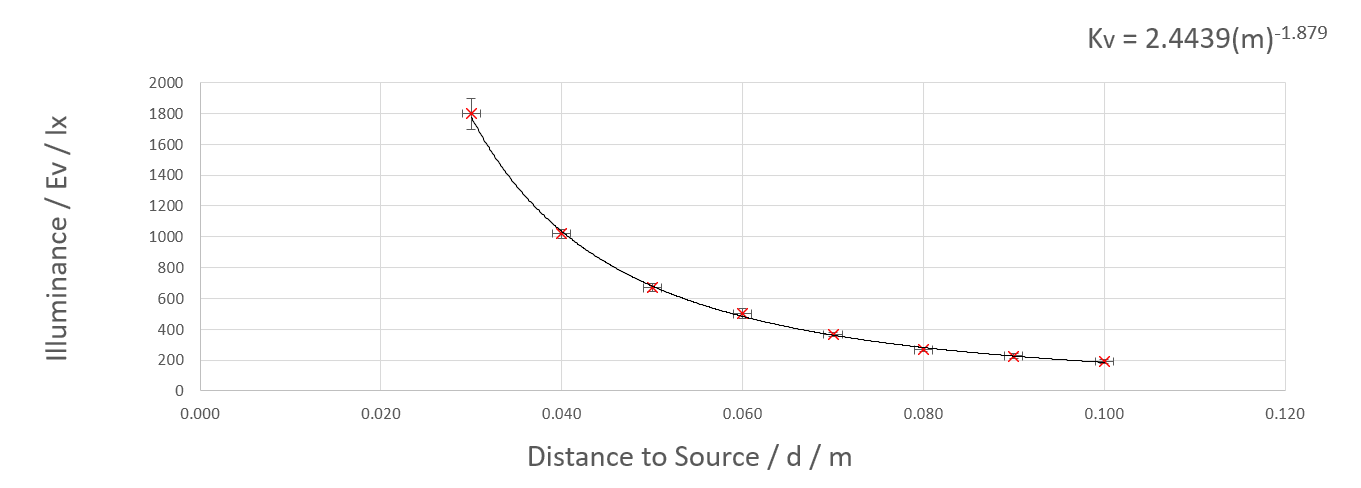
\includegraphics[width=\textwidth]{assets/averagegraph.png}
    \caption{Graph of the averaged illuminance values}
    \label{gph:average}
\end{figure}

Graph \ref{gph:average} looks like an inverse squared graph, attempt straightening with $1/{\text{distance}}^2$ transformation. The transformation data and error is generated with Microsoft Excel (figure \ref{fig:tdata}, graph \ref{gph:tdata}).

\textit{Error bars}: $\relun 1/{\text{distance}}^2$ = $2 \times \relun \text{distance}$

\begin{figure}
    \centering
    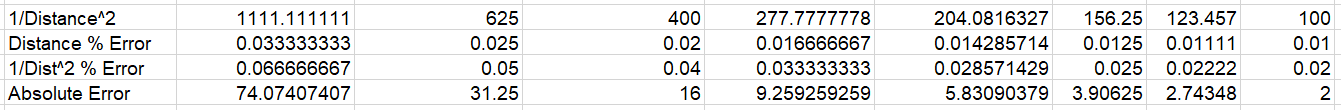
\includegraphics[width=\textwidth]{assets/transformdata.png}
    \caption{Transformed distance data}
    \label{fig:tdata}
\end{figure}

\begin{figure}
    \centering
    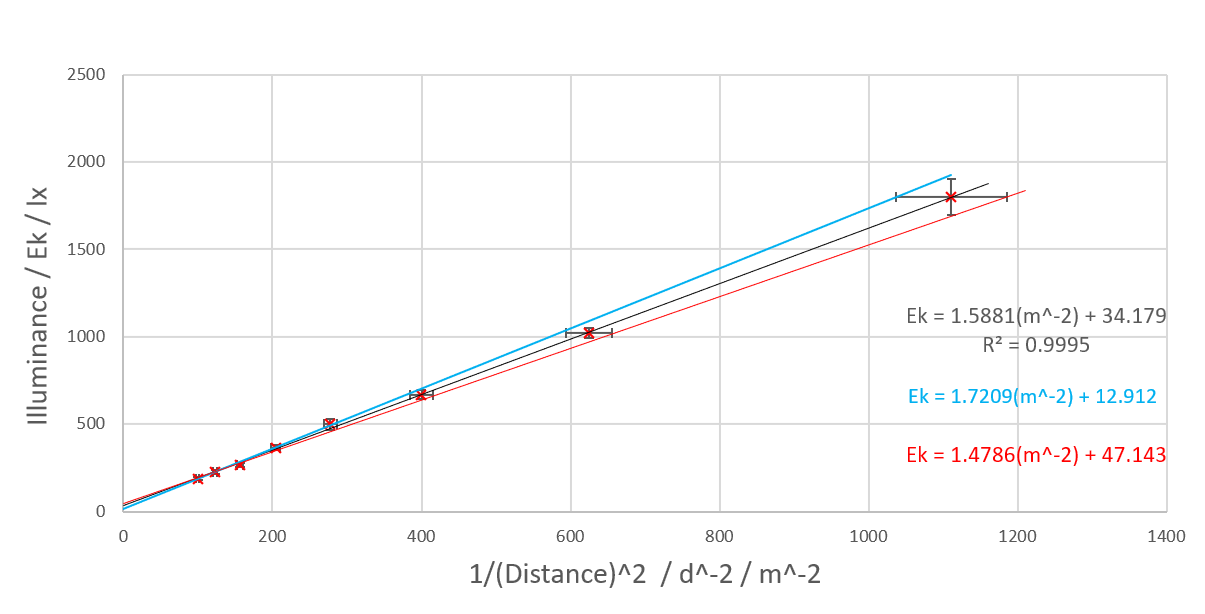
\includegraphics[width=\textwidth]{assets/transformgraph.png}
    \caption{Transformed distance graph}
    \label{gph:tdata}
\end{figure}

The two linear regression formulas from graph \ref{gph:tdata} are as follow:
\begin{align*}
    E_v &= 1.58 \frac{1}{s^2} + 49.2\\
    E_v &= 1.76 \frac{1}{s^2} - 25.5
\end{align*}

Final \% error: $|1.58-1.76| / 1.58 \approx 0.114 \approx 11.4\%$

\textit{Uncertainty}: 11.4\% of $1.58$ = 0.2 (1 sf)

Slope = $1.6 \pm 0.2$

Therefore, the equation is derived as figure \ref{fig:rel}:
\begin{figure}[h!]
    \[
       E_v = (1.6 \pm 0.2) \frac{1}{s^2} + 49.2
    \]
    \caption{Experimental relationship between illuminance against distance from source}
    \label{fig:rel}
\end{figure}

\section{Conclusions}
\subsection{Result}
\subsection{Implications}
\subsection{Reflection}

% other stuff

\newpage
\nocite{*}
\printbibliography



\end{document}
